\documentclass[UTF8]{ctexart}

\usepackage{WeeklyReport}
\usepackage{graphicx}
\usepackage{amsmath}
\usepackage{amssymb}

\title{周报09}
\author{傅阳烨}
\date{\today}

\begin{document}
\maketitle
% \tableofcontents
\section{学习内容}
\begin{itemize}
    \item 讨论 implicit alignment 在 MSDA 问题中的应用
    \item 阅读 Multi-View 相关文章
    \item 改进实验代码
\end{itemize}

\section{学习收获}
\subsection{Implicit Alignment}

与特征选取不同,在 Implicit Alignment 的文章中,作者的关注点在于处理不同域之间的类不平衡以及类分布漂移的问题。
在多源领域自适应中,类不平衡和漂移的问题也是存在的,但由于类不平衡的问题比较复杂,所以之前只讨论了特征对齐的问题,
下面来讨论 Implicit Alignment 在多源领域适应上面的应用。

文章给出的想法是,定义一些类集合的交集,差集等,研究其之间的关系。

对于两个域(假设类标签集合为 $A$ 和 $B$)的情况,只需要定义三个集合:$A \cap B$,$A - B$ 和 $B - A$,
分别称为共享标签和域特有的标签。在 input 上也定义了一些集合:
$\mathcal{B}_S^C:=\left \{ x\in \mathcal{B}_S \mid y\in Y_C \right \}$, $\mathcal{B}^{\overline{C}}_{S}:=\left \{ x\in \mathcal{B}_S \mid y\notin Y_C \right \}$, $\mathcal{B}_T^C:=\left \{ x\in \mathcal{B}_T \mid y\in Y_C \right \}$, $\mathcal{B}^{\overline{C}}_{T}:=\left \{ x\in \mathcal{B}_T \mid y\notin Y_C \right \}$,
其中 $Y_C = A \cap B$ 。

然后去判断数据来自哪个集合,属于域特有集合的样本可以直接被划分给对应的域。

而在多源的情况,集合的数量会随域的个数以指数级增长,在类标签方面,集合可以分为某一个域所特有的类,任意两个域所特有的类,
任意三个域所特有的类等情况,假设域标签的集合分别为 $S_1, S_2, \dots, S_n$,如果只考虑一个域所特有的类和所有域共有的类,则可以得到如下 $n+1$ 个集合:

$$
Y_i = S_i - \bigcup_{k \neq i}S_k,\quad i = 1, 2, \dots, n
$$

$$
Y = \bigcap_{i=1}^n S_i
$$

同样的,对于 input,也可以定义一系列集合:

$$
B_{S_i}^Y := \left\{x\in B_{S_i} | y\in Y\right\},\quad i = 1, 2, \dots, n
$$

$$
B_{S_i}^{\overline{Y}} := \left\{x\in B_{S_i} | y\notin Y\right\},\quad i = 1, 2, \dots, n
$$

然后再用前面的方法去判断域标签(相当于是绕过了学习域特有信息的过程)。

另外,文中提到了一种 mask 的方法,用来在训练的时候筛选属于某个域的部分,
在多源的情况,可以为每个域设定 mask 函数,但这只适用于所有源域和目标域的类标签已知的情况。
在特征选取的时候,特征的具体含义是模糊的,也就无法人为地确定某个特征是否是某个域独有的,
这个地方只能通过学习得到(比如用常见的加权的方式选取重叠特征)。

\subsection{Multi-View 论文阅读}
\subsubsection{Reciprocal Multi-Layer Subspace Learning for Multi-View Clustering (ICCV2019)}

\textbf{基本思路}

Multi-View 在处理高维数据,难以保留不同 view 之间的一致性和互补性。
文章提出 Reciprocal Multi-layer Subspace Learning (RMSL) 算法用于多视角聚类,主要由两部分组成:

\begin{enumerate}
    \item 层级化自表现层:Hierarchical Self-Representative Layers (HSRL)
    \item 反向编码网络:Backward Encoding Networks (BEN)
\end{enumerate}

Multi-View 的基本思想是在多个视角的数据中寻找共识(跟多源领域适应寻找共同特征很像),传统方法一般是直接将高维数据投影到同一个空间,
忽略了高维情况下不同 view 之间的不平衡性,造成聚类效果的下降。

子空间聚类目标在于获得数据根本上(underlying)的子空间结构,一般是寻找一个亲和性矩阵,
每一个 entry 揭露\underline{两个}样本的相似性程度(degree)。

对于一些 multi-view 子空间聚类的方法,可分为两类。第一类使用自表现方法(self-representation),
让每个视角分别去学习一个亲和性矩阵,将各个视角独有的亲和性矩阵合并,得到一个综合的相似性矩阵,
反映数据之间的固有联系。但是每个视角单独训练很难得到综合的信息,并且只能得到线性关系的子空间。
第二类主要是寻找一个不同视角之间共享的 latent space,然后在上面导出自表现(self-representation)。
但是这种方法又损失了不同视角的一致性(consistency),并且这个方法是在 raw-feature level 上集成多个视角的,
很容易受到数据的高维度和噪声的影响。

\begin{figure}[ht]
    \centering
    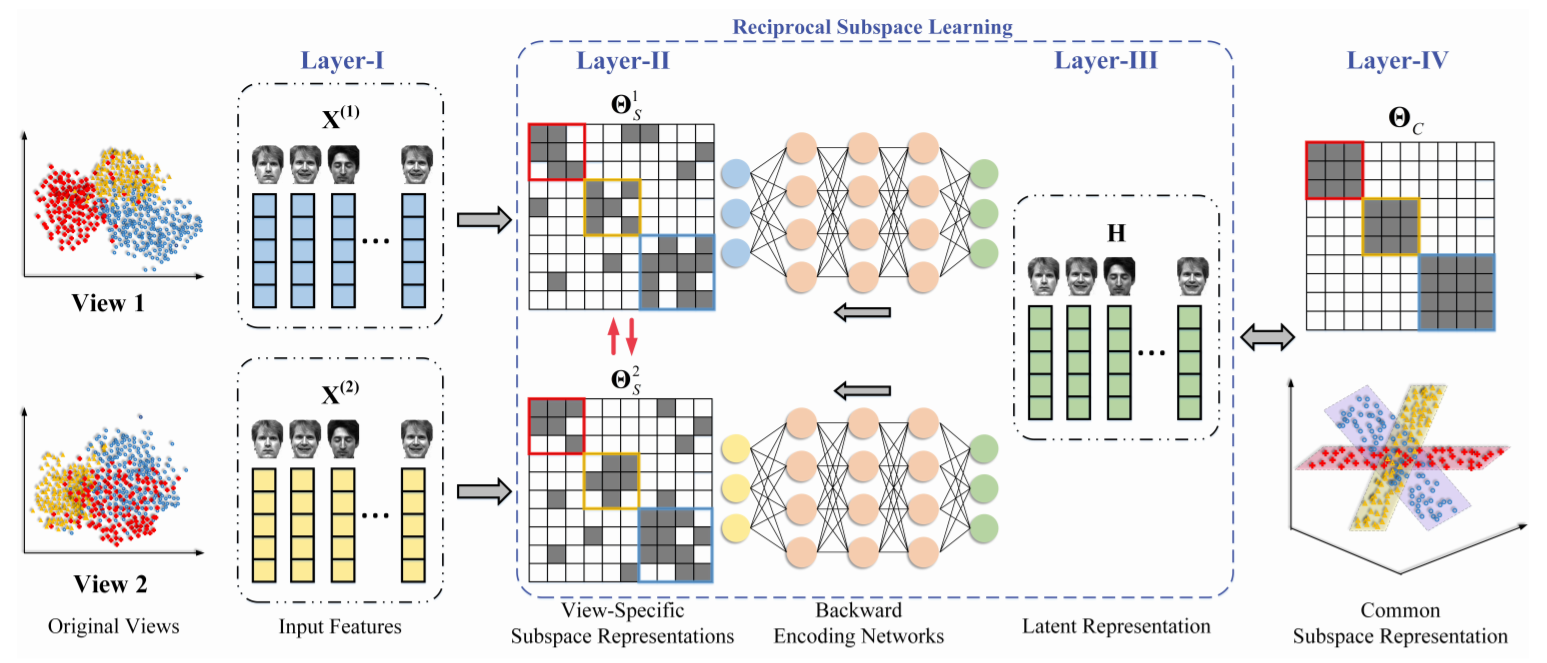
\includegraphics[scale=0.32]{Week09_RMSL.png}
    \caption{Reciprocal Multi-Layer Subspace Learning (RMSL) 结构}
    \label{fig:RMSL}
\end{figure}

文章提出了如图 \ref{fig:RMSL} 所示的 reciprocal multi-layer 子空间表示,
连接上 latent space $\mathbf{H}$,层级化地恢复(recover)数据的根本聚类结构,
多层的子空间表示可以互惠地在一个联合框架中相互提升。

BEN 从普通的 representation $\mathbf{H}$ 中重建视角各自的自表现,
使得 $\mathbf{H}$ 能够灵活地从多视角集成综合信息,反应数据点之间的固有联系。

在处理多视角时,先通过 BEN 进行 view-specific 的 subspace 的 encode,
得到 latent representation $\mathbf{H}$,避免了 raw-feature level 的集成。

\textbf{Hierarchical Self-Representation Layers}

在子空间聚类时,对于一组从多个子空间得到的数据点 $\mathbf{X} = \left[\mathbf{x_1}, \mathbf{x_2}, \dots, \mathbf{x_N}\right]$,
每一个可以表示为所有数据的一个线性组合($\mathbf{X} = \mathbf{X}\mathbf{Z}$),
其中 $\mathbf{Z}$ 是通过学习得到的自表现系数矩阵,优化方程如下:

$$
\min_{\mathbf{Z}}\mathcal{L}(\mathbf{X; \mathbf{Z}}) + \beta\mathcal{R}(\mathbf{Z})
$$

其中 $\mathcal{L}(\cdot; \cdot)$ 和 $\mathcal{R}(\cdot)$ 分别表示在 $\mathbf{Z}$ 上自表现的项(term)和规范化,
得到相似性矩阵 $S = |\mathbf{Z}| + |\mathbf{Z}^T|$。

$\mathcal{L}(\mathbf{X; \mathbf{Z}})$ 实际上可以看成没有激活层的全连接神经网络,$\mathbf{Z}$ 表示的是其参数。
假设 $\left\{\mathbf{X^1}, \mathbf{X^2}, \dots, \mathbf{X^V}\right\}$ 来自于 $V$ 个不同的视角,
$\mathbf{H}$ 表示 latent representation。使用 Hierarchical Self-Representation Layers (HSRL) 去构建 view-specific 和 common
的 subspace representation,分别用 $\{\Theta_S^v\}_{v=1}^V$ 和 $\Theta_C$ 表示。
使用 view-specific SRL 将原始数据映射到 subspace representation,common SRL 则更深入地揭露 latent representation $\mathbf{H}$ 的子空间结构。
对于 HSRL 的参数,使用如下方程进行优化:

$$
\min_{\{\Theta_S^v\}_{v=1}^V, \Theta_C} \mathcal{L}_S(\{\mathbf{X}^v\}_{v=1}^V, \mathbf{H};\{\Theta_S^v\}_{v=1}^V, \Theta_C) + \beta \mathcal{R}(\{\Theta_S^v\}_{v=1}^V, \Theta_C)
$$

其中 $\mathcal{L}_S(\cdot;\cdot)$ 表示与自表现相关的 loss function。

在文章中,对于重建 loss,使用了 Frobenius norm,对于 regularization 则使用了 nuclear norm,由此保证类内的高度同质性,
则上式被写为:

$$
\min_{\{\Theta_S^v\}_{v=1}^V, \Theta_C} \frac{1}{2}\sum_{v=1}^V\|\mathbf{X}^v-\mathbf{X}^v\Theta_S^v\|_F^2 + \frac{1}{2}\|\mathbf{H}-\mathbf{H}\Theta_C\|_F^2 + \beta(\sum_{v=1}^V\|\Theta_S^v\|_* + \|\Theta_C\|_*)
$$

\textbf{Backward Encoding Networks}

针对不同 view-specific 子空间表示之间的互补性,文章提出了 Backward Encoding Networks (BEN),以此得到 $\mathbf{H}$。
使用如下的 loss function 更新 BEN 的参数,得到 $\mathbf{H}$:

\begin{align*}
    &\min_{\{\Theta_E^v\}_{v=1}^V, \mathbf{H}} \mathcal{L}_E(\{\Theta_S^v\}_{v=1}^V, \mathbf{H}; \{\Theta_E^v\}_{v=1}^V) + \gamma\mathcal{R}(\{\Theta_E^v\}_{v=1}^V)\\
    =&\min_{\{\Theta_E^v\}_{v=1}^V, \mathbf{H}} \frac{1}{2}\sum_{v=1}^V\|\Theta_S^v-g_{\Theta_E^v}(\mathbf{H})\|_F^2 + \gamma\sum_{v=1}^V\|\Theta_E^v\|_F^2
\end{align*}

其中 $g_{\Theta_E^v}(\mathbf{H}) = \mathbf{W}_M^v f(\mathbf{W}_{M-1}^v \cdots f(\mathbf{W}_1^v \mathbf{H}))$,
$f$ 是激活函数,$\mathcal{L}_E$ 表示 $\mathbf{H}$ 的重建损失。BEN 总共包括 $M$ 个全连接层,将不同视角的互补信息 encode 到 common latent representation $\mathbf{H}$ 上,
$\mathcal{R}(\{\Theta_E^v\}_{v=1}^V)$ 是 regularization 项。

接下来,整个 RMSL 的参数,包括 BEN 和 HSRL,可以用以下目标函数联合优化得到:

$$
\min_{\mathbf{H},\Theta} \alpha \mathcal{L}_E(\{\Theta_S^v\}_{v=1}^V, \mathbf{H}; \{\Theta_E^v\}_{v=1}^V) + \gamma\mathcal{R}(\{\Theta_E^v\}_{v=1}^V) + \mathcal{L}_S(\{\mathbf{X}^v\}_{v=1}^V, \mathbf{H};\{\Theta_S^v\}_{v=1}^V, \Theta_C) + \beta \mathcal{R}(\{\Theta_S^v\}_{v=1}^V, \Theta_C)
$$

\textbf{Experiments}

\begin{figure}[ht]
    \centering
    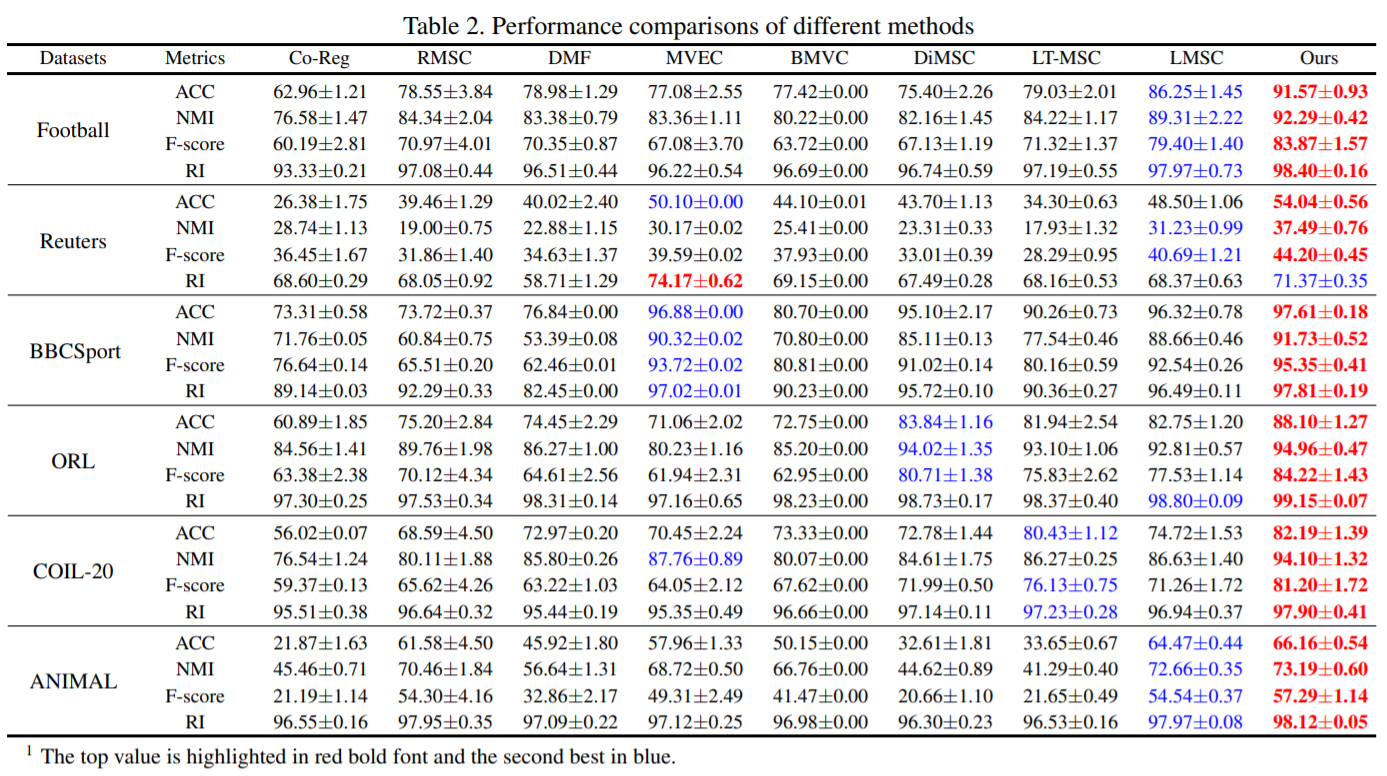
\includegraphics[scale=0.32]{Week09_RMSL_test.png}
    \caption{RMSL 的实验结果}
    \label{fig:RMSLtest}
\end{figure}

作者在 Football、Reuters、BBCSport、ORL、COIL-20 和 ANIMAL 六个数据集上进行了实验,得到的结果如图 \ref{fig:RMSLtest} 所示。

从实验结果可以看出,论文中提出的方法在各个数据集上都比原先的结果有显著的提升,
说明 RMSL 进行子空间提取的方式是有效的。

\subsection{实验(MSDA 在 DomainNet 上的测试)}

找到了文章的附加材料,在里面仍然没有讲 DomainNet 的实现和架构细节,但是提到了图像放缩的尺寸是 224 x 224,以及训练的 batch size 是 16。

在代码上的改动需要重新写一下特征提取器和分类器,以及图片在读取时的放缩大小改为 224 x 224,训练的 batch size 改为 16,
其它的结构暂时保持与 Digit-Five 的实验一致,训练部分的代码也需要做相应的调整。

现在代码还没有改好,之后改好了再做实验看看效果如何。

\section{启发}
\begin{enumerate}
    \item RMSL 的思想与我最先对于多源特征提取的想法非常相似,都是找到不同域(或者视角)之间的数据互补性,可以尝试把原模型特征提取的部分改换成 RMSL 的结构,用 common subspace representation 去表示特征
\end{enumerate}
\section{疑问/困难}
\begin{enumerate}
    \item 多源领域适应中的类不平衡的问题仍然比较复杂,之后可能还是把关注点放在多源特征提取和匹配上(假定所有域都相同的类标签)
    \item 对于 Alternating Direction Minimization 的优化过程不太理解,在论文中使用了增强型拉格朗日乘子(Augmented Lagrange Multiplier)的方法,但并没有看懂
    \item RMSL 所提供的代码是 matlab 的,不能直接放在 pytorch 里面使用
\end{enumerate}
\end{document}
